\documentclass[dvipdfmx]{jsarticle}
\usepackage[dvipdfmx]{graphicx}
\usepackage{float}
\usepackage{listings}

\lstset{%
  language={C},
  basicstyle={\small},%
  identifierstyle={\small},%
  commentstyle={\small\itshape},%
  keywordstyle={\small\bfseries},%
  ndkeywordstyle={\small},%
  stringstyle={\small\ttfamily},
  frame={tb},
  breaklines=true,
  columns=[l]{fullflexible},%
  numbers=left,%
  xrightmargin=0zw,%
  xleftmargin=3zw,%
  numberstyle={\scriptsize},%
  stepnumber=1,
  numbersep=1zw,%
  lineskip=-0.5ex%
}

\renewcommand{\lstlistingname}{プログラム}


\begin{document}

\title{アドバンスドCG第1回}
\author{日比野 文}
\maketitle

\section*{課題1}

\lstinputlisting[caption=.frag]{/home/pomu/sagyo/3d/myapp/GLSL/scene01\_checker2D.frag}
\lstinputlisting[caption=.vert]{/home/pomu/sagyo/3d/myapp/GLSL/scene01\_checker2D.vert}
\begin{figure}[H]
 \begin{center}
  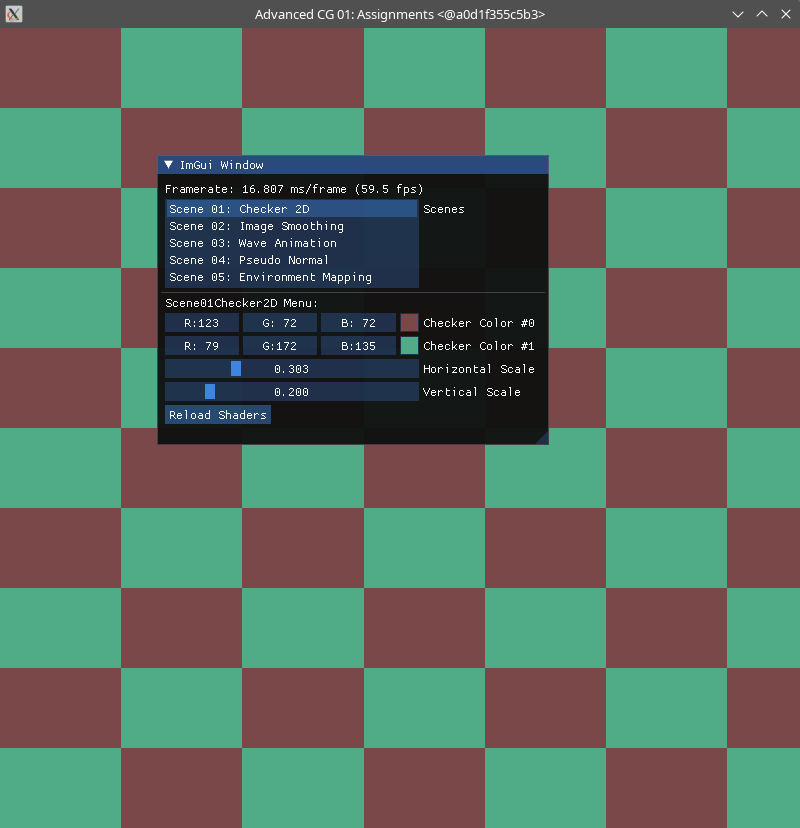
\includegraphics[width=10cm]{/home/pomu/sagyo/tex/advancedCG/figures/kadai1.png}
 \end{center}
 \caption{課題1}
 \label{fig:kadai1}
\end{figure}

\section*{課題2}
%\lstinputlisting[caption=.frag]{/home/pomu/sagyo/3d/myapp/GLSL/scene02_image_smoothing.frag}
%\lstinputlisting[caption=.vert]{/home/pomu/sagyo/3d/myapp/GLSL/scene02_image_smoothing.vert}
%\begin{figure}[H]
% \begin{center}
%  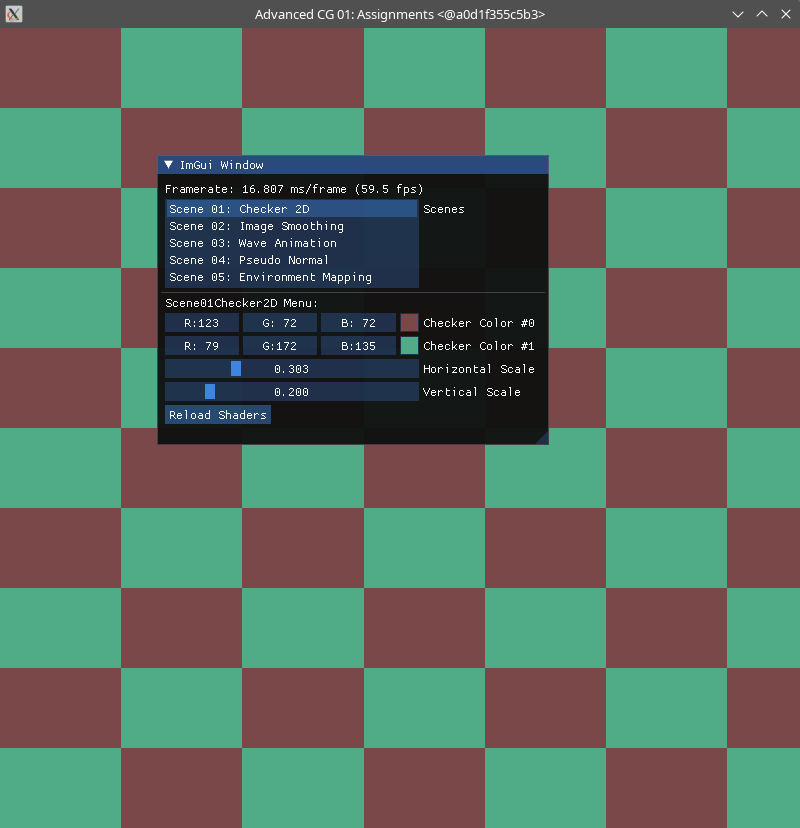
\includegraphics[width=10cm]{/home/pomu/sagyo/tex/advancedCG/figures/kadai1.png}
% \end{center}
% \caption{課題1}
% \label{fig:kadai1}
%\end{figure}
完成できませんでした。

\section*{課題3}
\lstinputlisting[caption=.frag]{/home/pomu/sagyo/3d/myapp/GLSL/scene03_wave_animation.frag}
\lstinputlisting[caption=.vert]{/home/pomu/sagyo/3d/myapp/GLSL/scene03_wave_animation.vert}
\begin{figure}[H]
 \begin{center}
  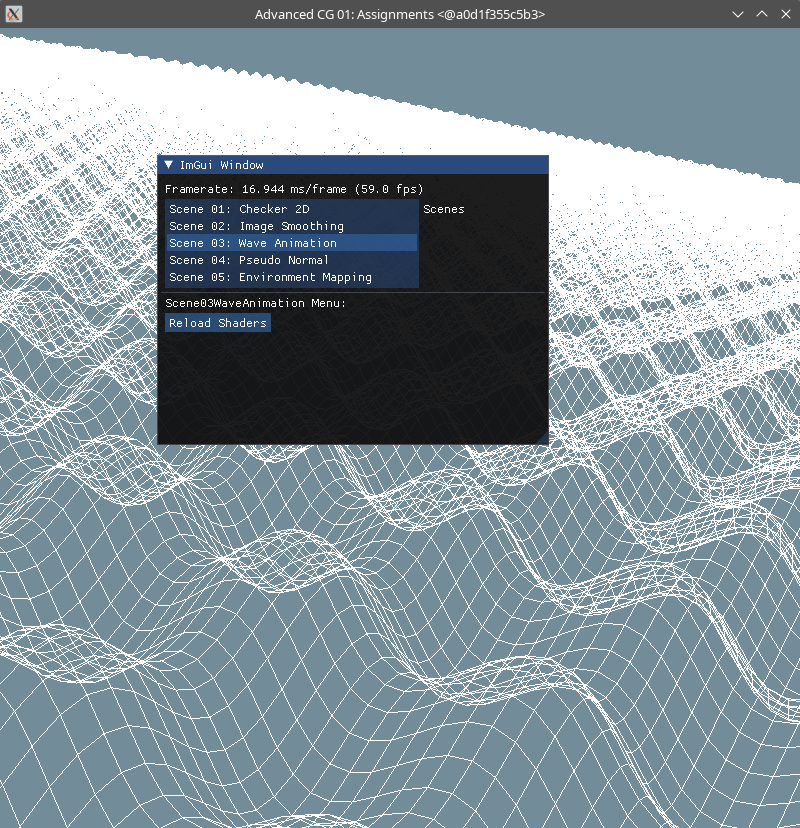
\includegraphics[width=10cm]{/home/pomu/sagyo/tex/advancedCG/figures/kadai3.png}
 \end{center}
 \caption{課題3}
 \label{fig:kadai1}
\end{figure}

\section*{課題4}
\lstinputlisting[caption=.frag]{/home/pomu/sagyo/3d/myapp/GLSL/scene04_pseudo_normal.frag}
\lstinputlisting[caption=.vert]{/home/pomu/sagyo/3d/myapp/GLSL/scene04_pseudo_normal.vert}
\begin{figure}[H]
 \begin{center}
  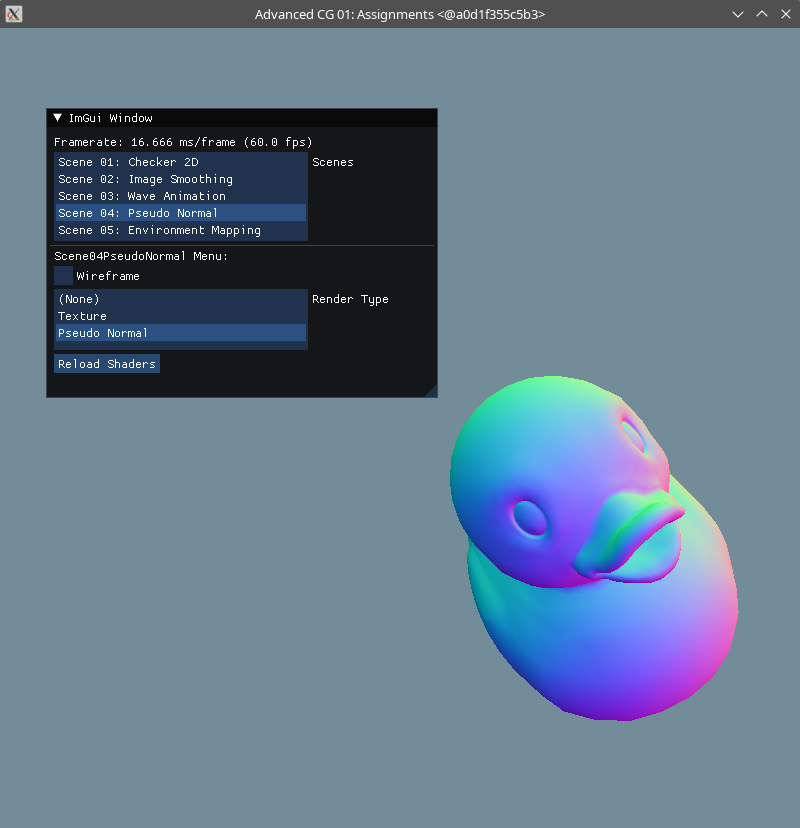
\includegraphics[width=10cm]{/home/pomu/sagyo/tex/advancedCG/figures/kadai4.png}
 \end{center}
 \caption{課題4}
 \label{fig:kadai1}
\end{figure}

\section*{課題5}
\lstinputlisting[caption=.frag]{/home/pomu/sagyo/3d/myapp/GLSL/scene05_envmap.frag}
\lstinputlisting[caption=.vert]{/home/pomu/sagyo/3d/myapp/GLSL/scene05_envmap.vert}
\begin{figure}[H]
 \begin{center}
  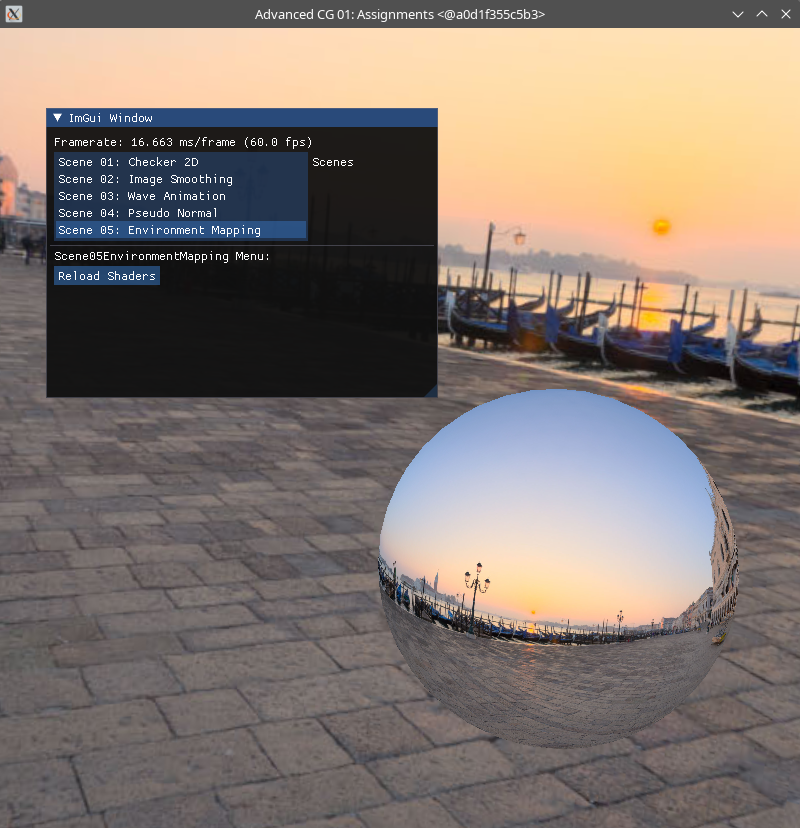
\includegraphics[width=10cm]{/home/pomu/sagyo/tex/advancedCG/figures/kadai5.png}
 \end{center}
 \caption{課題5}
 \label{fig:kadai1}
\end{figure}

\section*{動作環境}
dockerで作成したdebian上で動作させた。
\lstinputlisting[caption=Dockerfile]{/home/pomu/sagyo/3d/Dockerfile}
\lstinputlisting[caption=Makefile]{/home/pomu/sagyo/3d/Makefile}
ホスト環境は以下の通り。\\
OS:slackware 15.1\\
\begin{lstlisting}[caption=uname -aの実行結果]
Linux aya.home 6.1.57 #1 SMP PREEMPT_DYNAMIC Tue Oct 10 23:06:41 CDT 2023 x86_64 AMD Ryzen Threadripper 1950X 16-Core Processor AuthenticAMD GNU/Linux\\
\end{lstlisting}

\end{document}
